\section{Animacije}
Igre se većinom rade tako da korisnik upravlja sa nekim objektom. Da bi taj objekt bio vizualno zanimljiv potrebno mu je dodati neke animacije. Animacije se u Unity-u rade u animacijskom prozoru. Animacijski prozor sadrži vremensku crtu koja nam služi da odredimo vrijeme animacije. Jedan objekt može imati više animacija.
Sučelje za kontrolu svih animacija objekta se zove Animator kontrola.

\subsection{Animator kontrola}
Sa animator kontrolom određujemo kada će se koja animacija izvršiti. Najčešće je slučaj da objekt ima više animacija koje čekaju svoj red za izvršavanje. Animator kontrola tu postavlja redosljed izvršavanja animacija. Npr. ukoliko je određena animacija aktivna i kad korisnik pritisne određenu tipku ta animacija prelazi na drugu određenu animaciju. Na slici je prikazana animator kontrola za objekt "Player". 


\begin{center}
	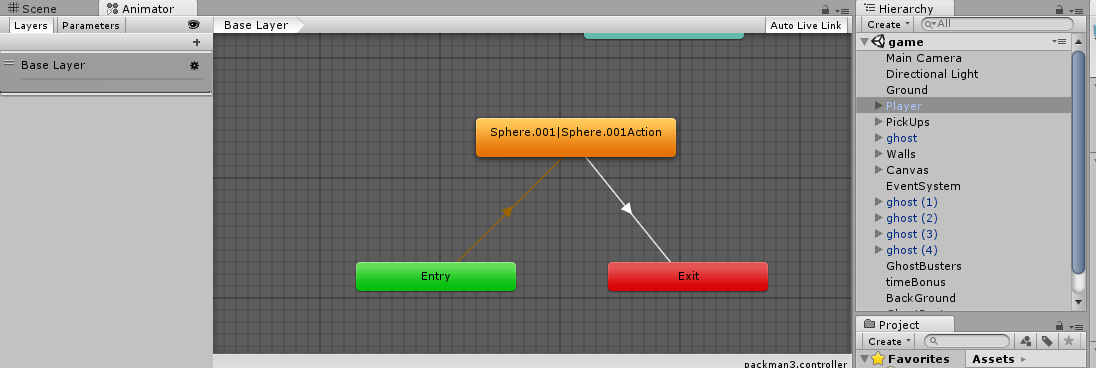
\includegraphics[scale=0.60]{animacijaPrimjer.png}
	
	
	Slika 7: Dodjeljivanje animacija objektu
\end{center}